
\documentclass[11pt]{article}


\usepackage[pdftex]{graphicx}
\usepackage{url} 
\usepackage[dvips, bookmarks, colorlinks=false, pdfborder={0 0 0}, pdftitle={<pdf title here>}, pdfauthor={<author's name here>}, pdfsubject={<subject here>}, pdfkeywords={<keywords here>}]{hyperref} 
\usepackage[final]{pdfpages}
\usepackage{multirow}


\title{XSM \\ eXperimental String Machine \\
Version 1.0}
\author{Dr. K. Muralikrishnan  \\ \texttt{kmurali@nitc.ac.in} \\ {NIT Calicut} }


\begin{document}

\maketitle
\pagebreak

%......................Table of Contents............................%
\thispagestyle{plain}

\tableofcontents
\pagebreak


\section{Introduction}

\subsection{Brief Machine Description}
The machine simulator is known as Experimental String Machine (XSM). It is an interrupt driven uniprocessor machine. The machine handles data as 16 byte strings. A string is a sequence of characters terminated by '\textbackslash 0'. The length of a string is atmost 15 characters. The machine interprets a single character also as a string.

\subsection{Components of the Machine}

\begin{figure}[hbtp]
\begin{center}
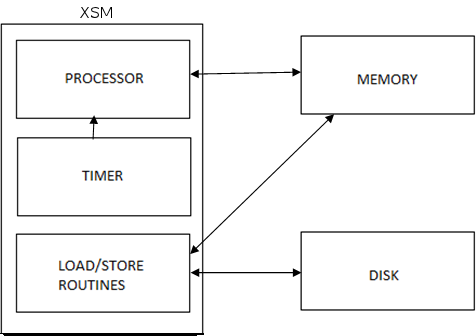
\includegraphics[scale=0.5]{block.png}
\end{center}
\caption{Components of the Machine}
\end{figure}


\begin{itemize}
\item Disk : It is a non-volatile storage that stores user programs (executables) and data files.
\item Memory : It is a volatile storage that stores the programs to be run on the machine as well as the operating system that manages the various programs.
\item Processor : It is the main computational unit that is used to execute the instructions.
\item Timer : It is a device that interrupts the processor after a pre-defined specific time interval.
\item Load/Store : It is a macro that performs the functionalities of DMA (Direct Memory Access) controller.
\end{itemize}






\section{Registers}

\subsection{Introduction}
The XSM architecture maintains 24 string registers.

\subsection{Register Set}
There are 16 General Purpose Registers (GPR), R0 - R15, of which R0 - R7 are Program Registers and R8 - R15 are Kernel Registers. There are 4 temporary registers T0 - T3 which are reserved for code translation. These registers cannot be used by the system programmer. In addition to these 20 registers there are 4 special purpose registers BP, IP, SP and PID which are used as Base Pointer, Instruction Pointer, Stack Pointer and Process Identifier respectively.\\


\begin{center}
\begin{tabular}{|c|c|}
\hline Name & Register \\ 
\hline Program Register & R0-R7 \\ 
\hline Kernel Register & R8-R15 \\ 
\hline Temporary Registers & T0-T3 \\ 
\hline Base Pointer & BP \\ 
\hline Instruction Pointer & IP \\ 
\hline Stack Pointer & SP \\ 
\hline Process Identifier & PID \\ 
\hline 
\end{tabular} 
\end{center}

\section{Memory}

\subsection{Introduction}

%\begin{figure}[hbtp]
%\begin{center}
%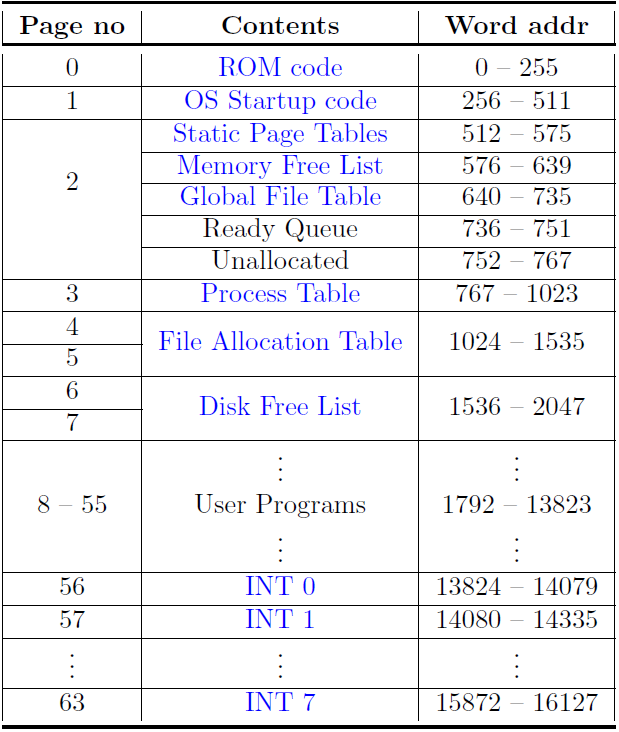
\includegraphics[scale=0.5]{memoryblockdiagram.png}
%\end{center}
%\caption{Main Memory Block Diagram}
%\end{figure}

\begin{itemize}
\item The basic unit of memory in XSM is a 16 byte string.
\item The machine memory can be thought of as a linear sequence of strings.
\item A collection of 256 contiguous strings is known as a page.
\item The total size of the memory is 64 pages or 16384 (256 $\times$ 64) strings.
\item Each string in the memory is identified by the \textit{string address} in the range 0 to 16383(256 $\times$ 64 - 1). Similarly, each page in the memory is identified by the \textit{page number} in the range 0 to 63.
\end{itemize}
\textbf{
\subsection{Address Translation}}

There are two kinds of memory addresses,\\

\begin{itemize}
\item Logical address : When a process runs, CPU generates address for the data accessed by this process. This address is called the Logical address.

\item Physical address : It is the actual location of the data in the main memory.
\end{itemize}

Address translation is the process of obtaining the physical address from the logical address. It is done by the machine in the following way. 
\begin{enumerate}
\item The logical address generated by the CPU is divided by the page size (256) to get the \textbf{logical page number}. The remainder is the \textbf{offset} of the data within that page.


\item A \textbf{page table} is used for address translation. It contains physical page numbers corresponding to each logical page number. The logical page number is used to index the page table to get the corresponding physical page number.

\item The \textbf{offset} is then used to refer to the word in the physical page containing the data.
\end{enumerate}






\section{File System}
\subsection{Introduction}

\textbf{Block} : It is the basic unit of storage in the disk.\\
The disk can be thought of as consisting of a linear sequence of 512 blocks. The size of each block isequal to that of a page in the memory (256 words).

\subsection{Disk Structure}
The basic structure of the disk is shown in figure below.

\begin{figure}[hbtp]
\begin{center}
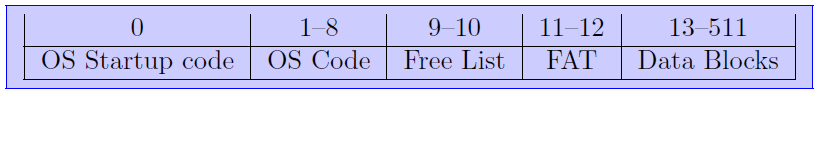
\includegraphics[scale=0.5]{fileblockdiagram.png}
\end{center}
\caption{Structure of the disk}
\end{figure}


\subsection{Addressing}
\textbf{Block number} : Any particular block in the disk is addressed by the corresponding number in the sequence 0 to 511 known as the block number.

\subsection{Disk Free List}
\begin{itemize}
\item The Free List of the disk consists of 512 entries. Each entry is of size one word.
\item The total size of the free list is thus 2 blocks or 512 words (512(= no. of entries) x 1(= size of one entry) = 512 words).
\item It is present in blocks 9 and 10 of the disk.
\item Each entry of the free list contains a value of either 0 or 1 indicating whether the corresponding block in the disk is free or not respectively.
\end{itemize}


\subsection{File}
A file is a collection of data identified by a name. Every file in the disk has a Basic Block and several Data Blocks. They are defined as follows:
\begin{itemize}
\item Data Blocks : These blocks contain the actual data of a file.
\item Basic Block : It consists of information about the data of a file.Composed of Block List and Header.
 
 \begin{figure}[hbtp]
\begin{center}
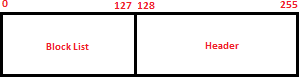
\includegraphics[scale=0.5]{fileblock.png}
\end{center}
\caption{Structure of a Basic Block of a file}
\end{figure}
\begin{itemize}
 \item Block List : It is similar to an index in a book which tells which chapter starts from which page.The block list consists of 128 entries each of size one word.The value contained in an entry of the block list gives the block number of the corresponding data block in the disk.
 \item Header : The header contains the header information relating to the file. Currently this is unused, but at a later stage can be used to store information such as file modification date/time, author of the file etc.
 
 \end{itemize}
\end{itemize}


\subsubsection{File Types}
There are two types of files in the XSM architecture. They are:
\begin{enumerate}
\item Data files : These files contain data or information that is used by the programs. They can occupy a maximum of 129 blocks (1 basic block + 0 - 128 data blocks).
\item Executable files : These contain programs that the user wishes to run on the machine. They occupy 3 blocks (1 basic block + 2 data blocks) of the disk.
\end{enumerate}


\subsubsection{Executable File Format}

It consists of the Code section which contains the actual code to be run on the machine. It can span upto a maximum of 2 blocks.


\subsection{File Allocation Table (FAT)}
File allocation table (FAT) is a table that has an entry for each file present in thedisk.
\begin{itemize}
\item FAT of the filesystem consists of 32 entries. Thus there can be a maximum of 32 files.
\item Each entry is of size 16 words.
\item Total size of the FAT is thus 512 words (32 (= number of entries) x 16(= size of one entry) = 512 words).
\item It is a disk data structure and occupies block numbers 11 and 12 of the disk.
\end{itemize}

\subsubsection{Structure of a FAT entry}

\begin{figure}
\begin{center}
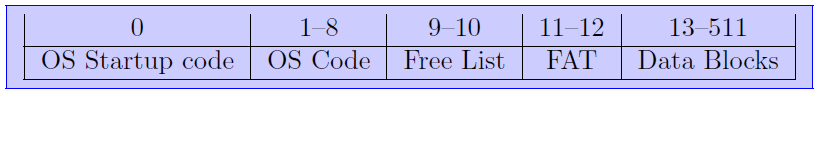
\includegraphics[scale=0.5]{fileblockdiagram.png}
\end{center}
\caption{Structure of a FAT entry}
\end{figure}

\begin{enumerate}
\item File Name : It is an identification of a file. It can be of maximum 15 characters (and thus requires 1 word). Typical file names are student.txt, calc.sim.
\item File size : It indicates the number of words occupied by a file. It varies from 0 words to (128 x 256) words (depending upon the number of data blocks it has). It occupies one word in the FAT entry.
\item Block number of basic block : It contains the block number where the basic block of a file resides in the disk. It occupies one word in the FAT entry.
\end{enumerate}



\pagebreak

\section{Process}

\subsection{Introduction}
\textbf{Process} : Any program written by the user is run as a process by the kernel.
\begin{itemize}
\item The XSM architecture supports a maximum of 12 processes to be run at a time.
\item Each process is allowed to occupy a maximum of 4 pages of the memory.
\end{itemize}

\subsection{Process Structure}
Any process in the memory has the following structure.
\begin{itemize}
\item Code Area : These are pages of the memory that contain the actual code to be run on the machine. It occupies 2 pages of the memory.
\item Stack : This is the user stack used in program execution. It is used to pass arguments during function calls, storing activation record of a function etc. It occupies 2 pages of the memory and grows in the direction of increasing word address.
\end{itemize}

\subsection{Registers Associated with a Process}

\begin{itemize}
\item Every process is allotted a unique integer identifier in the range 0 to 15, known as the PID (Process Identifier) which is stored in the PID register. This register can be used as an operand in any instruction only when executing in the kernel mode.
\item The word address of the currently executing instruction is stored in the IP (Instruction Pointer) register. This register can be used as an operand in any instruction only when executing in the kernel mode.
\item The base address of the user stack is stored in the BP (Base Pointer) register.
\item The address of the stack top is stored in the SP (Stack Pointer) register. Each process has its own set of values for the various registers.
\end{itemize}


\subsection{Data Structures Associated with a Process}
The following are the various data structures associated with a process. They are explained in the following subsections.

\subsubsection{Process Control Block (PCB)}
It contains data pertaining to the current state of the process.
Note that the size of each PCB (Process Control Block) is 16 words.

\begin{figure}
\begin{center}
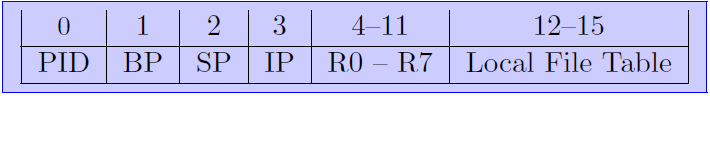
\includegraphics[scale=0.5]{pcbblockdiagram.png}
\end{center}
\caption{Structure of Process Control Block}
\end{figure}

\subsubsection{The Page Table}
The page table stores the exact location in the memory of the data related to a process.
\begin{itemize}
\item Each process has 4 entries in the page table.
\begin{itemize}
\item zeroth entry corresponds to the first page of code area.
\item first entry corresponds to the second page of code area.
\item third and fourth entry corresponds to the stack.
\end{itemize}
\item Each entry contains the page number where the data specified by the logical address resides in the memory.
\end{itemize}


\subsubsection{Page Tables}
The page tables of the 12 processes are stored in the first 48 words of page 2 of the memory. 
\begin{itemize}
\item The size of each page table is 4 words ( 4(= no. of entries) x 1(= size of an entry)= 4 words).
\item There are a total of 12 processes, thus accounting for the 48 words( 12 X 4 words).
\item The page tables are indexed by multiplying the PID of a process by the size of a page table to get the starting word address of the page table of that process.
\end{itemize}

\subsubsection{Process Table}
\begin{itemize}
\item The process table contains the PCB of each of the 12 processes (Each entry occupies 16 words).
\item The page 3 of the memory contains the process table.
\item There are a total of 12 processes, thus accounting for the 192 words (12 × 16 words).
\item The process table is indexed by multiplying the PID of a process by the size of a PCB to get the starting word address of the PCB of that process.
\end{itemize}



\section{Instructions}

\subsection{Introduction}
The instructions provided by the XSM architecture can be classified into privileged and unprivileged instructions.

\subsection{Classification}

\subsubsection{Unprivileged Instructions}
\begin{enumerate}
\item MOV
\begin{itemize}
\item Immediate Addressing:\\
\textit{Syntax :} MOV Ri, NUM/STRING
\item Register Addressing:\\
\textit{Syntax :} MOV Ri, Rj\\
Source register - Ri, Destination register - Rj
\item Register Indirect Addressing:\\
\textit{Syntax }: MOV Ri, [Rj]\\
Copy contents of memory location pointed by Rj to Ri.\\
\textit{Syntax :} MOV [Ri], Rj \\
Contents of Rj are copied to the location whose address is in Ri.
\item Direct Addressing:\\
\textit{Syntax :} MOV [LOC], Rj\\
Contents of Rj are transferred to the address LOC.\\
\textit{Syntax :} MOV Rj, [LOC]\\
Contents of the memory location LOC are transferred to Rj.
\end{itemize}


\item Arithmetic Instructions

\begin{itemize}
\item ADD, SUB, MUL, DIV and MOD.\\
\textit{General Syntax :} OP Ri, Rj\\
The result of Ri op Rj is stored in Ri. If Ri and/or Rj are not integers, these instructions does no operation.
\item INR\\
\textit{Syntax :} INR Rj\\
Increments the value of register Rj by one.
\item  DCR\\
\textit{Syntax :} DCR Rj
Decrements the value of register Rj by one.\\
Here Ri, Rj may be any registers except SP, BP and IP.
\end{itemize}


\item Logical Instructions
\begin{itemize}
\item LT\\
Syntax : LT Ri, Rj\\
Stores 1 in Ri if the value stored in Ri is less than that in Rj. Ri is set to 0 otherwise.
\item GT\\
Syntax : GT Ri, Rj\\
Stores 1 in Ri if the value stored in Ri is greater than that in Rj. Ri set to 0 otherwise.
\item EQ\\
Syntax : EQ Ri, Rj\\
Stores 1 in Ri if the value stored in Ri is equal to that in Rj. Set to 0 otherwise.Here content of Ri and Rj can be strings also.
\item NE\\
Syntax : NE Ri, Rj\\
Stores 1 in Ri if the value stored in Ri is not equal to that in Rj. Set to 0 otherwise.Here content of Ri and Rj can be strings also.
\item GE\\
Syntax : GE Ri, Rj\\
Stores 1 in Ri if the value stored in Ri is greater than or equal to that in Rj. Set to 0 otherwise.
\item LE\\
Syntax : LE Ri, Rj\\
Stores 1 in Ri if the value stored in Ri is less than or equal to that in Rj. Set to 0 otherwise.\\
Here Ri, Rj may be any registers except SP, BP and IP.
\end{itemize}

\item Branching Instructions\\
Branching is achieved by changing the value of the IP to the address of a specified LABEL. 
\begin{itemize}
\item JZ\\
Syntax : JZ Ri, LABEL\\
Jumps to LABEL if the contents of Ri is zero.
\item JNZ\\
Syntax : JNZ Ri, LABEL\\
Jumps to LABEL if the contents of Ri is not zero.
\item JMP\\
Syntax : JMP LABEL\\
Unconditional Jump to instruction specified at LABEL\\
Here Ri can be any register except SP, BP and IP.
\end{itemize}

\item Stack Instructions
\begin{itemize}
\item PUSH\\
Syntax : PUSH Ri\\
Increment SP by 1 and copy contents of Ri to the location pointed to by SP.
\item POP\\
Syntax : POP Ri\\
Copy contents of the location pointed to by SP into Ri and decrement SP by 1.\\
For both these instructions Ri may be any register except IP.
\end{itemize}

\item Subroutine Instructions\\
The CALL instruction copies the address of the next instruction to be fetched (IP + 1) on to the stack, and transfers control to the label specified. The RET instruction restores the IP value stored in the stack and continues execution fetching the next instruction pointed to by IP. The subroutine instructions provide a neat mechanism for procedure evocations.
\begin{itemize}
\item CALL\\
Syntax : CALL LABEL\\
Increment SP by 1, transfers IP+1 to location pointed to by SP and jumps to LABEL
\item RET\\
Syntax : RET\\
Sets IP to the value pointed to by SP and decrements SP.
\end{itemize}

\item Input/Output Instructions
\begin{itemize}
\item IN\\
Syntax : IN Ri\\
Transfers the contents of the standard input to Ri.
\item OUT\\
Syntax : OUT Ri\\
Transfers the contents of Ri to the standard output.\\
Ri can be any register except IP, BP and SP.
\end{itemize}

\item START\\
IP will be initialised to this instruction automatically when a program is taken for execution.
\item END\\
Syntax : END\\
This instruction is put at the end of a user program.
\item INT\\
Syntax : INT no\\
This instruction generates an interrupt to the kernel with no as a parameter.
\end{enumerate}


\subsubsection{Privileged Instructions}
There are four privileged instructions. They are:
\begin{enumerate}
\item IRET\\
Syntax : IRET\\
This instruction pops the return address from the user stack of the process which invoked the interrupt and assigns it to the IP register. IRET does the same action as RET, but it tells the processor that the interrupt handler has finished. With the execution of the IRET instruction, interrupts are enabled.
\item LOAD\\
Syntax : LOAD pg\textunderscore no block\textunderscore no\\
This instruction loads the block specified by the block\textunderscore no, from the disk, to the page specified by the pg\textunderscore no, in the memory. block\textunderscore no and page\textunderscore no can be numbers or registers containing numbers.
\item STORE\\
Syntax : STORE block\textunderscore no pg\textunderscore no\\ 
This instruction stores the page specified by the pg\textunderscore no, from the memory, to the block specified by the block\textunderscore no, in the disk. block\textunderscore no and page\textunderscore no can be numbers or registers containing numbers.
\item HALT\\
Syntax : HALT\\
This instruction causes the simulator to halt immediately.
\end{enumerate}

\subsection{Processor Modes}
The XSM architecture is interrupt driven and uses a single processor. There are two modes of operation, the user mode and the kernel mode.
\begin{itemize}
\item User mode : All unprivileged instructions can be executed in this mode.
\item Kernel mode : Both privileged and unprivileged instructions can be executed in this mode. The processor comes to know about the mode in which the system is running by looking at the value in the IP register.
\end{itemize}


\section{Interrupts}

\subsection{Introduction}
Interrupts are mechanisms by which the user code interrupts the execution of the processor and passes control to the kernel to accomplish low level functionalities like disk access, arithmetic exception handling etc.\\
\textbf{Interrupt Service Routine(ISR)} : The kernel provides routines to accomplish the functionality for which an interrupt has been generated. These routines are known as Interrupt Service Routines.\\
Note: Every ISR should end with an IRET instruction.

\subsection{The INT instruction}
The instruction used to generate an interrupt is INT.\\
Syntax : INT n\\
The INT instruction passes control to the Interrupt Service Routine (ISR) for this interrupt located at the physical address computed using the value n.
Address computation is done as follows. The physical address of the ISR corresponding to interrupt number n is given by:
Physical Address = (56 + n) × Page Size
Note that the interrupts are disabled once this instruction is executed, since we do not allow interrupts to occur in kernel mode.

\subsection{Types of Interrupts}
There are 8 interrupts (numbered from 0 to 7) supported by the SSM architecture. The interrupts 0 and 7 are hardware interrupts and the remaining interrupts (1 to 6) are software interrupts.\\
Details of hardware interrupts are as follows.
\begin{itemize}
\item INT 0 : This is the timer interrupt which interrupts the processor forcing a context switch. It contains the code for the scheduler of the operating system, which schedules the CPU time among the various active processes. Note that this interrupt cannot be called from the user/kernel mode.
\item INT 7 : It is generated when the following exceptions1 occur:
\begin{enumerate}

%CHECK THE ADDRESSES

\item Illegal memory access : occurs when any address generated by the process does not lie in the range [0, 959].
\item Arithmetic exception : occurs when divisor is 0.
\item Illegal instruction : occurs when an attempt is made to execute an instruction not belonging to the instruction set and also when the operands to the instruction is not legal. Eg: MOV 4 R0, MOV IP 4 when executed in user mode. These instructions are considered illegal.
\item Stack overflow and stack underflow : Stack overflow occurs when the value in the SP register exceeds 959 and stack underflow occurs when the value falls below 768.
\end{enumerate}
\item INT 1, INT 2 : These interrupts are used for the various file system calls. 
\item INT 3, INT 4 : These interrupts are used for the various process system calls. 
\item INT 5, INT 6 : These interrupts have been kept reserved for future use.The interrupts 1, 2, 3 and 4 are unprivileged and can be called from user mode.
\end{itemize}


\end{document}